\documentclass[aspectratio=169]{beamer}

% <<< BEGIN tema

\usetheme[nomyriadpro,progressbar]{unam}

% logos (los valores por defecto ya apuntan a assets/; se pueden cambiar aquí)
\unammotto{}
\unamslidelogo{
\includegraphics[width=0.45\paperheight]{assets/unam-escudo-gris}}

% portada: escudo más grande, ocupando el espacio sobre el título
\unamtitlelogo{
\includegraphics[height=0.5\paperheight]{assets/unam-escudo-gris}}
\makeatletter
\defbeamertemplate{background}{unamtitlebig}
{
    \begin{tikzpicture}[remember picture, overlay]
        \node [shading=axis, rectangle,
               left color=UNAMDarkBlue, right color=UNAMLightBlue!70,
               shading angle=45, anchor=north,
               minimum width=\paperwidth, minimum height=\paperheight]
               (box) at (current page.north) {};
        \node [opacity=0.5, anchor=north, yshift=-0.3cm] at (current page.north)
            {\unam@titlelogo};
    \end{tikzpicture}
}
% pie de página: GitHub en lugar de www.unam.mx
\defbeamertemplate{footline}{unamgithub}{
    \vspace{5pt}
    \ifunam@progressbar
    \unam@progressbarwidth=\paperwidth
    \multiply\unam@progressbarwidth by \insertframenumber
    \divide\unam@progressbarwidth by \inserttotalframenumber
    \begin{tikzpicture}[remember picture, overlay]
    \fill[UNAMGold, anchor=west]
        (0, -0.3ex) rectangle (\unam@progressbarwidth, 0ex);
    \end{tikzpicture}%
    \fi
    \begin{beamercolorbox}[wd=\textwidth, ht=2.5ex]{footline hline}%
    \hfill \unam@motto
    \unam@mottospacing

    \hspace{\beamer@leftmargin}%
    \usebeamerfont{author in head/foot}\insertshortauthor%
    \hfill\usebeamercolor[fg]{url text}\usebeamerfont{url text}%
    \href{https://github.com/jairferrara}{github.com/jairferrara}%
    \hspace{1.75\beamer@rightmargin}
    \vspace*{0.75pt}
    \end{beamercolorbox}
    \begin{beamercolorbox}[wd=\textwidth, sep=5pt]{footline}%
        \centering
        \usebeamertemplate*{frame footer}
        \usebeamercolor[fg]{page number in head/foot}
        \usebeamerfont{page number in head/foot}
        \insertframenumber~/~\inserttotalframenumber
    \end{beamercolorbox}
}
\setbeamertemplate{footline}[unamgithub]
\makeatother
\RenewDocumentCommand \titleframe {} {
    \setbeamertemplate{title page}[unamtitlepage]
    \setbeamertemplate{background}[unamtitlebig]
    \frame[plain,noframenumbering]{\titlepage}
    \setbeamertemplate{background}[unamslide]
}

% presentación corta: sin diapositivas separadoras de sección
\AtBeginSection{}
% título largo: fuente un poco más chica en la portada
\setbeamerfont{title}{size=\large, series=\bfseries}

% sin símbolos de navegación
\beamertemplatenavigationsymbolsempty

% cómo se muestran los elementos ocultos: invisible / transparent / dynamic
\setbeamercovered{transparent}
\setbeamersize{text margin left=1.2em,text margin right=1.2em}
\addtobeamertemplate{frametitle}{}{\vspace{0.2em}}

% >>> END

% <<< BEGIN paquetes y macros

\usepackage{amsmath,amssymb,mathtools}
\usepackage{physics}
\usepackage{bm}
\usepackage{booktabs}
\usepackage{xcolor}
\usepackage{hyperref}
\usepackage[utf8]{inputenc}
\usepackage[T1]{fontenc}
\DeclareFontShape{T1}{cmss}{b}{n}{<->ssub*cmss/bx/n}{}
\DeclareFontShape{T1}{cmss}{m}{sc}{<->ssub*cmr/m/sc}{}

% gráficos con TikZ
\usepackage{tikz}
\usetikzlibrary{fit, backgrounds, arrows.meta, positioning}

% carpeta de imágenes
\graphicspath{{images/}}

\definecolor{myblue}{RGB}{30,100,180}
\definecolor{myred}{RGB}{180,30,30}
\definecolor{mygreen}{RGB}{20,140,60}
\definecolor{mypurple}{RGB}{120,30,160}
\definecolor{myorange}{RGB}{220,120,0}

% macros de ejemplo (agregar las propias del proyecto aquí)
\newcommand{\kv}{\mathbf{k}}
\newcommand{\etal}{\textit{et al.}}

% >>> END

% <<< BEGIN metadatos

\title[Estimadores de $\xi(r)$ y dilución de materia oscura]{Estudio sobre los estimadores de la función de correlación para modelos de dilución de materia oscura}
\subtitle[Propuesta de proyecto final]{Propuesta de proyecto final}
\author[J. Ferrara]{Jair Ferrara}
\institute{Universidad Nacional Autónoma de México}
\date{18 de noviembre de 2026}

% >>> END

\newcommand{\DD}{\mathrm{DD}}
\newcommand{\DR}{\mathrm{DR}}
\newcommand{\RR}{\mathrm{RR}}

\begin{document}

\titleframe

% ====================================================
\section{Objetivos}
% ====================================================

\begin{frame}{Objetivos}
  \textbf{General:} estudiar la covarianza de los estimadores de la función
  de correlación $\xi(r)$ en modelos de dilución de materia oscura, siguiendo
  el enfoque de Wang \& Steele, con campos gaussianos.

  \vspace{0.6em}
  \textbf{Objetivos ilustrativos:}
  \begin{enumerate}
    \item Resolver el crecimiento lineal $D_+$, $D_\Psi$ y $f_v=f+g$ para el
      benchmark de dilución $g(z)$.
    \item Generar realizaciones de campos gaussianos y catálogos con y sin
      dilución ($g=0$ vs.\ $g\neq0$).
    \item Medir $\hat\xi(r)$ y su matriz de covarianza a partir de las
      realizaciones; compararla con la predicción gaussiana.
    \item Explorar si la diferencia entre ambos modelos es significativa
      frente al error estadístico.
  \end{enumerate}
\end{frame}

% ====================================================
\section{Motivación}
% ====================================================

\begin{frame}{Motivación}
  \begin{columns}[T]
    \begin{column}{0.55\textwidth}
      \begin{itemize}
        \item En $\Lambda$CDM plano, el $\Omega_m$ inferido de BAO de
          \textbf{DESI DR2} es menor que el de \textbf{Planck} (CMB).
        \item No es evidencia de intercambio de energía en el sector oscuro,
          pero motiva preguntar si parte de lo atribuido a la energía oscura
          viene de un cambio en la \alert{materia}.
        \item Modelos con la misma expansión de fondo pueden tener
          \emph{clustering} distinto $\Rightarrow$ las perturbaciones
          rompen la degeneración.
        \item ¿Es la señal detectable? Hace falta conocer la
          \alert{covarianza} de los estimadores.
      \end{itemize}
    \end{column}
    \begin{column}{0.42\textwidth}
      \centering
      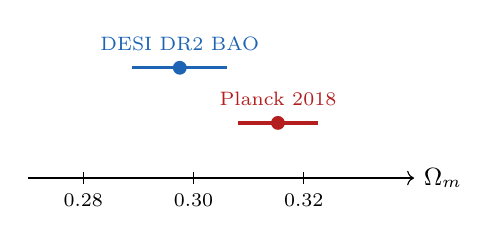
\begin{tikzpicture}[x=70cm, y=1cm]
        \draw[->] (0.27,0) -- (0.34,0) node[right, font=\small] {$\Omega_m$};
        \foreach \x in {0.28,0.30,0.32}
          \draw (\x,0.08) -- (\x,-0.08) node[below, font=\scriptsize] {\x};
        % DESI DR2 BAO
        \draw[myblue, very thick] (0.2975-0.0086,1.4) -- (0.2975+0.0086,1.4);
        \fill[myblue] (0.2975,1.4) circle (2.5pt);
        \node[myblue, font=\scriptsize, above] at (0.2975,1.5) {DESI DR2 BAO};
        % Planck 2018
        \draw[myred, very thick] (0.3153-0.0073,0.7) -- (0.3153+0.0073,0.7);
        \fill[myred] (0.3153,0.7) circle (2.5pt);
        \node[myred, font=\scriptsize, above] at (0.3153,0.8) {Planck 2018};
      \end{tikzpicture}

      \vspace{0.3em}
      {\scriptsize $\Omega_m = 0.2975\pm0.0086$ (DESI DR2)\\
      $\Omega_m = 0.315\pm0.007$ (Planck 2018)}
    \end{column}
  \end{columns}
\end{frame}

% ====================================================
\section{Punto de partida}
% ====================================================

\begin{frame}{Punto de partida}
  \begin{columns}[T]
    \begin{column}{0.5\textwidth}
      \textbf{Continuidad modificada:}
      \[
        \dot\rho + 3H\rho + \nabla\!\cdot(\rho\,\dot{\mathbf{x}}) = S,
        \qquad S = -g(t)H\bar\rho\,\delta
      \]
      \textbf{Crecimiento lineal} de la materia:
      \[
        \ddot D_+ + 2H(1+\Theta)\dot D_+
        - \tfrac32\Omega_m H^2 (1+\Xi) D_+ = 0
      \]
      \vspace{-0.6em}
      {\small $\Theta = g/2$, \ $\Xi = \Xi(g,\dot g)$; \ $g=0 \Rightarrow \Lambda$CDM.}
    \end{column}
    \begin{column}{0.47\textwidth}
      \textbf{Efecto en $P(k)$ a orden lineal:}
      \[
        P_{\rm dil}(k) = \left[\frac{D_+^{\rm dil}}{D_+^{\Lambda{\rm CDM}}}\right]^2
        P_{\Lambda{\rm CDM}}(k)
      \]
      \begin{itemize}
        \item Solo suprime la amplitud: misma forma y mismo BAO.
      \end{itemize}
    \end{column}
  \end{columns}
  \begin{block}{}
    \small Base: A.~Avilés \& J.~Ferrara, \textit{Dark Matter Dilution} (borrador).
  \end{block}
\end{frame}

% ====================================================
\section{Entradas}
% ====================================================

\begin{frame}{Entradas: modelo de juguete}
  \begin{itemize}
    \item \textbf{Benchmark del borrador:} fondo $\Lambda$CDM plano,
      $\Omega_{m0}=0.3$, con
      \[
        g(z) = \frac{g_0}{2}\left[1 - \tanh\!\left(\frac{z-z_t}{\Delta z}\right)\right],
        \quad g_0=0.2,\; z_t=2,\; \Delta z=0.2 .
      \]
    \item \textbf{Espectro lineal} $P_L(k)$ (CAMB, como en la práctica 04),
      reescalado con $D_+$ de cada modelo.
    \item \textbf{Campos gaussianos hechos a mano} en una caja periódica (FFT):
      $\delta_0(\mathbf{k}) \to \delta^{(1)},\ \Psi^{(1)},\ \mathcal{M}^{(1)}$.
    \item \textbf{Catálogos:} partículas desplazadas (Zel'dovich con $D_\Psi$)
      con peso $\mathcal{M}$; catálogos aleatorios para los estimadores.
    \item Muchas realizaciones con semillas distintas $\Rightarrow$ covarianza muestral.
  \end{itemize}
\end{frame}

% ====================================================
\section{Salidas}
% ====================================================

\begin{frame}{Salidas esperadas}
  \alert{Por definir con más detalle}; la idea es observar:
  \begin{itemize}
    \item $\hat\xi(r)$ (Landy--Szalay y otros) para $g=0$ y $g\neq0$.
    \item Matrices de covarianza y de correlación entre bins de $r$.
    \item Comparación entre covarianza muestral y predicción gaussiana
      (Wang \& Steele).
    \item Cómo cambian el ruido y la covarianza con el número de
      realizaciones, de aleatorios y el ancho de bin.
  \end{itemize}
\end{frame}

% ====================================================
\section{Plan de implementación}
% ====================================================

\begin{frame}{Plan de implementación}
  \centering
  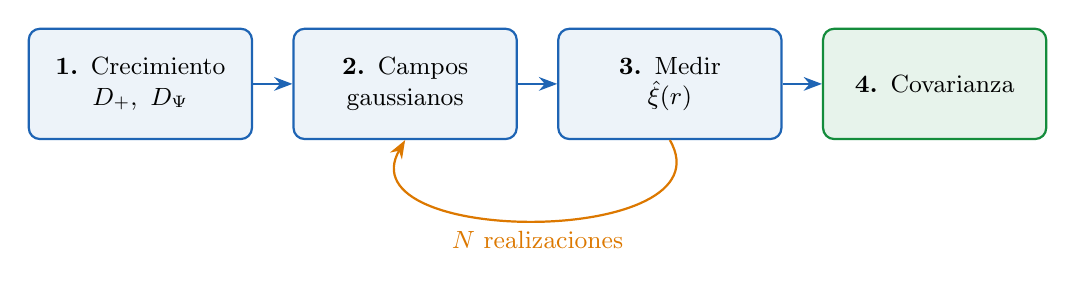
\begin{tikzpicture}[
      box/.style={draw=myblue, thick, rounded corners, fill=myblue!8,
        align=center, minimum height=1.4cm, text width=2.6cm, font=\small},
      arr/.style={-{Stealth}, thick, myblue}]
    \node[box] (a) {\textbf{1.} Crecimiento\\$D_+,\ D_\Psi$};
    \node[box, right=0.5cm of a] (b) {\textbf{2.} Campos\\gaussianos};
    \node[box, right=0.5cm of b] (c) {\textbf{3.} Medir\\$\hat\xi(r)$};
    \node[box, right=0.5cm of c, fill=mygreen!10, draw=mygreen] (d)
      {\textbf{4.} Covarianza};
    \draw[arr] (a) -- (b); \draw[arr] (b) -- (c); \draw[arr] (c) -- (d);
    \draw[arr, myorange] (c.south) to[out=-60, in=-120, looseness=1.2]
      node[below, font=\small] {$N$ realizaciones} (b.south);
  \end{tikzpicture}

  \vspace{1em}
  \raggedright\small
  Se compara $g=0$ vs.\ $g\neq0$, y la covarianza muestral vs.\ la gaussiana.\\[0.4em]
  \alert{Por investigar:} la covarianza de Wang \& Steele con pesos $\mathcal{M}$.
\end{frame}

% ====================================================
\section{Bibliografía}
% ====================================================

\begin{frame}{Bibliografía}
  \begin{block}{Trabajo base}
    \small
    \begin{itemize}
      \item A.~Avilés \& J.~Ferrara, \textit{Dark Matter Dilution: A Two-Field Lagrangian
        Perturbation Theory of Large-Scale Structure}, borrador (en preparación).
    \end{itemize}
  \end{block}
  \vspace{0.3em}
  \begin{exampleblock}{Semilla}
    \small
    \begin{itemize}
      \item DESI Collaboration (M.~Abdul-Karim \etal), \textit{DESI DR2 Results II:
        Measurements of BAO and Cosmological Constraints}, arXiv:2503.14738.
      \item Planck Collaboration (N.~Aghanim \etal), \textit{Planck 2018 results.
        VI. Cosmological parameters}, A\&A \textbf{641} (2020) A6, arXiv:1807.06209.
    \end{itemize}
  \end{exampleblock}
\end{frame}

% ---- cierre: con fondo de sección ----
\section{¡Gracias! \texorpdfstring{\\[0.4em]}{} {\normalsize ¿Preguntas y comentarios?}}
\sectionframe

\end{document}
